% $Id: introduction.tex 87303 2016-02-08 13:44:29Z lafferty $

\subsection{Fit model}
\label{subsec:fit}
Only events in the BDT range [0.6,1] are considered in the fit to the data.
A simultaneous fit to the mass distribution across four equally-sized
independent bins of the BDT response is performed. The combinatorial background is described
with an exponential \pdf for both FULL and PARTIAL analysis, with independent floating yields and
decay constants in each BDT bin. The signal
model is an Hypathia distribution~\cite{Ipatia} with different configurations
for FULL and PARTIAL (see \figref{fig:Ipatia}). The signal model parameters are independent
in each BDT bin and are obtained from simulation. The fractions of signal events allotted to each
BDT bin are also fixed from values obtained from simulation, with a total signal yield remaining as the sole free parameter describing signal in the simultaneous fit. %%%\textcolor{red}{J: What do you do with the background?}
The signal yield is floated in the fit to the data. It is measured to be 
compatible with zero within one to two sigma. %, given the limited size of the data sample.
The fit projections to the FULL and PARTIAL data are shown in \figref{fig:fit}.% and \figref{fig:fitPARTIAL},respectively.
\begin{figure} [htb!]
\begin{center}
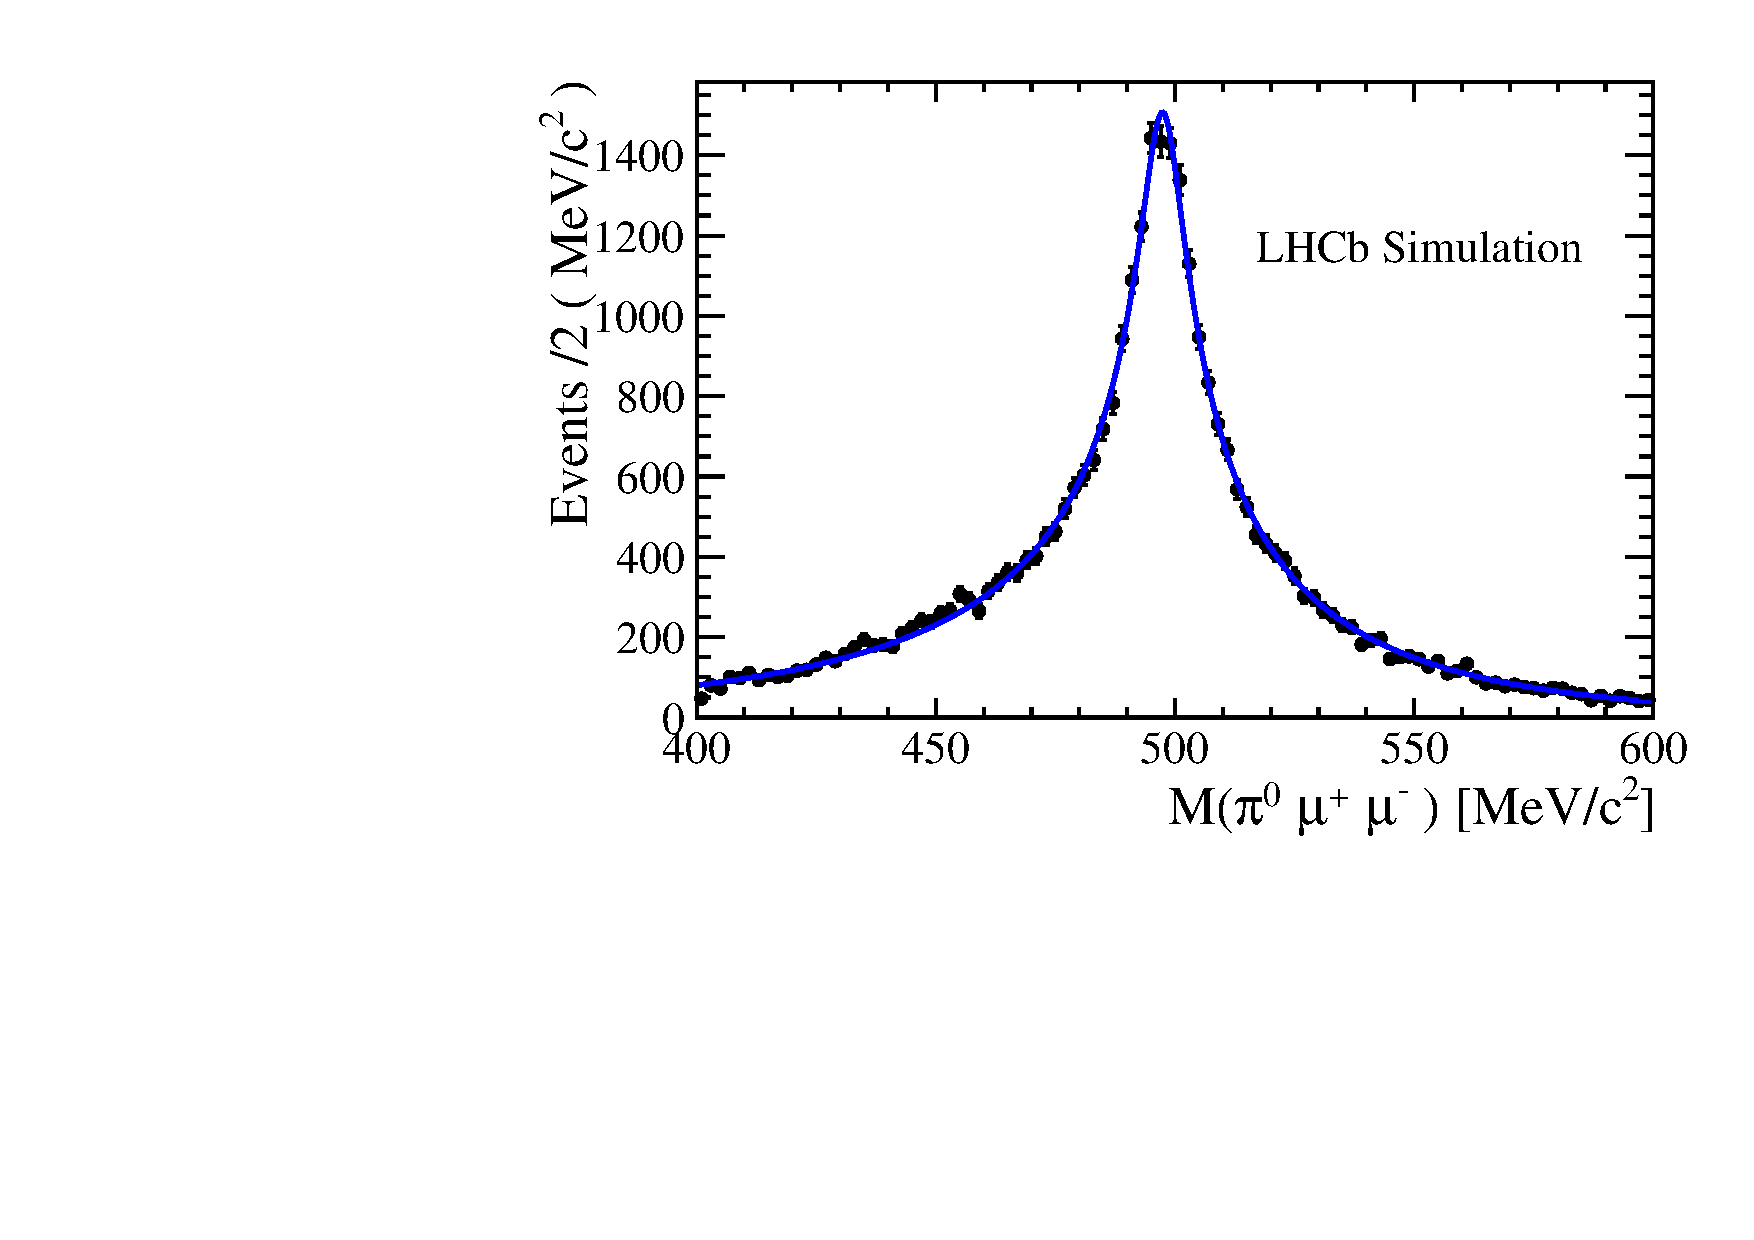
\includegraphics[scale=0.30]{figs/Kspi0MuMu/Ipatia_pi0.pdf}
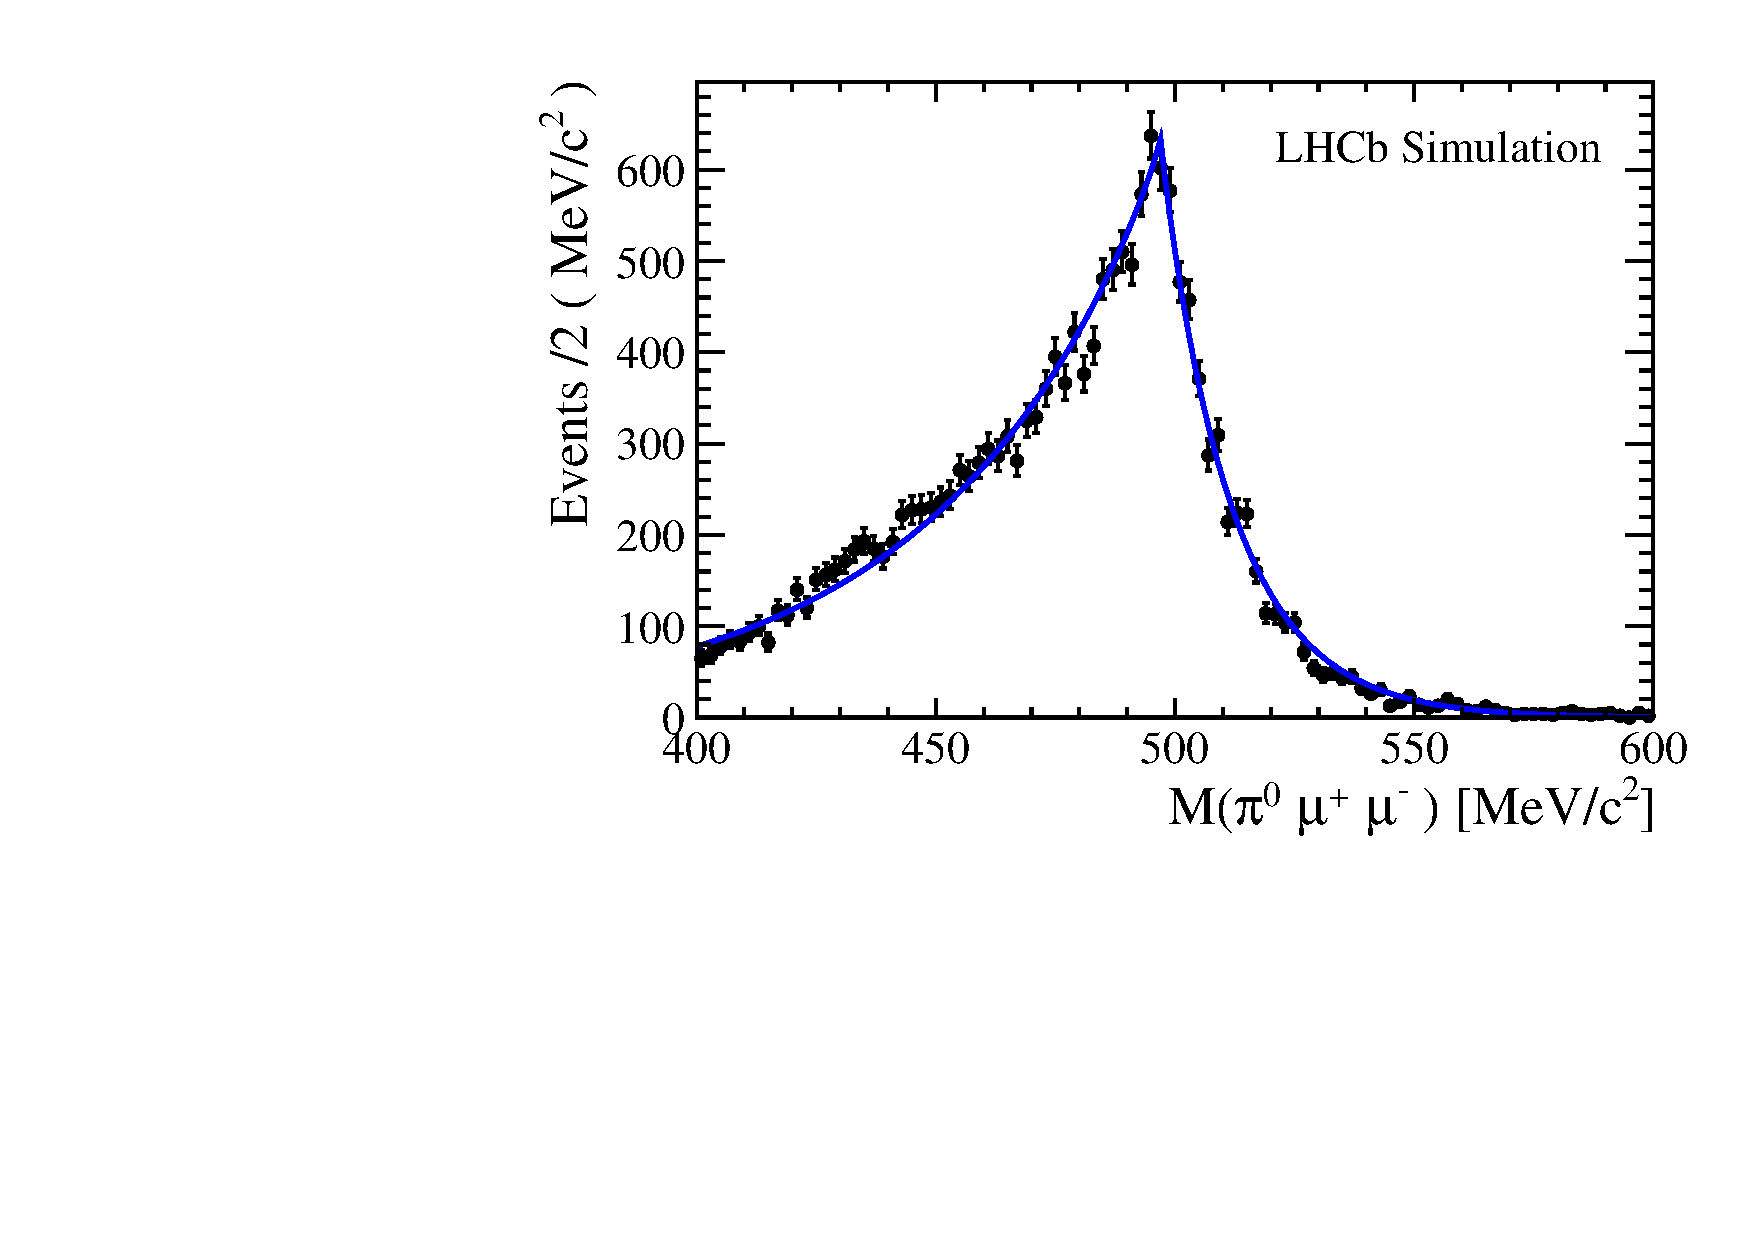
\includegraphics[scale=0.30]{figs/Kspi0MuMu/Ipatia_nopi0.pdf}
\caption{Signal fit using the Hypathia function for FULL (left) and PARTIAL (right) categories. \label{fig:Ipatia}}
\end{center}
\end{figure}

\begin{figure} [htb!]
\begin{center}
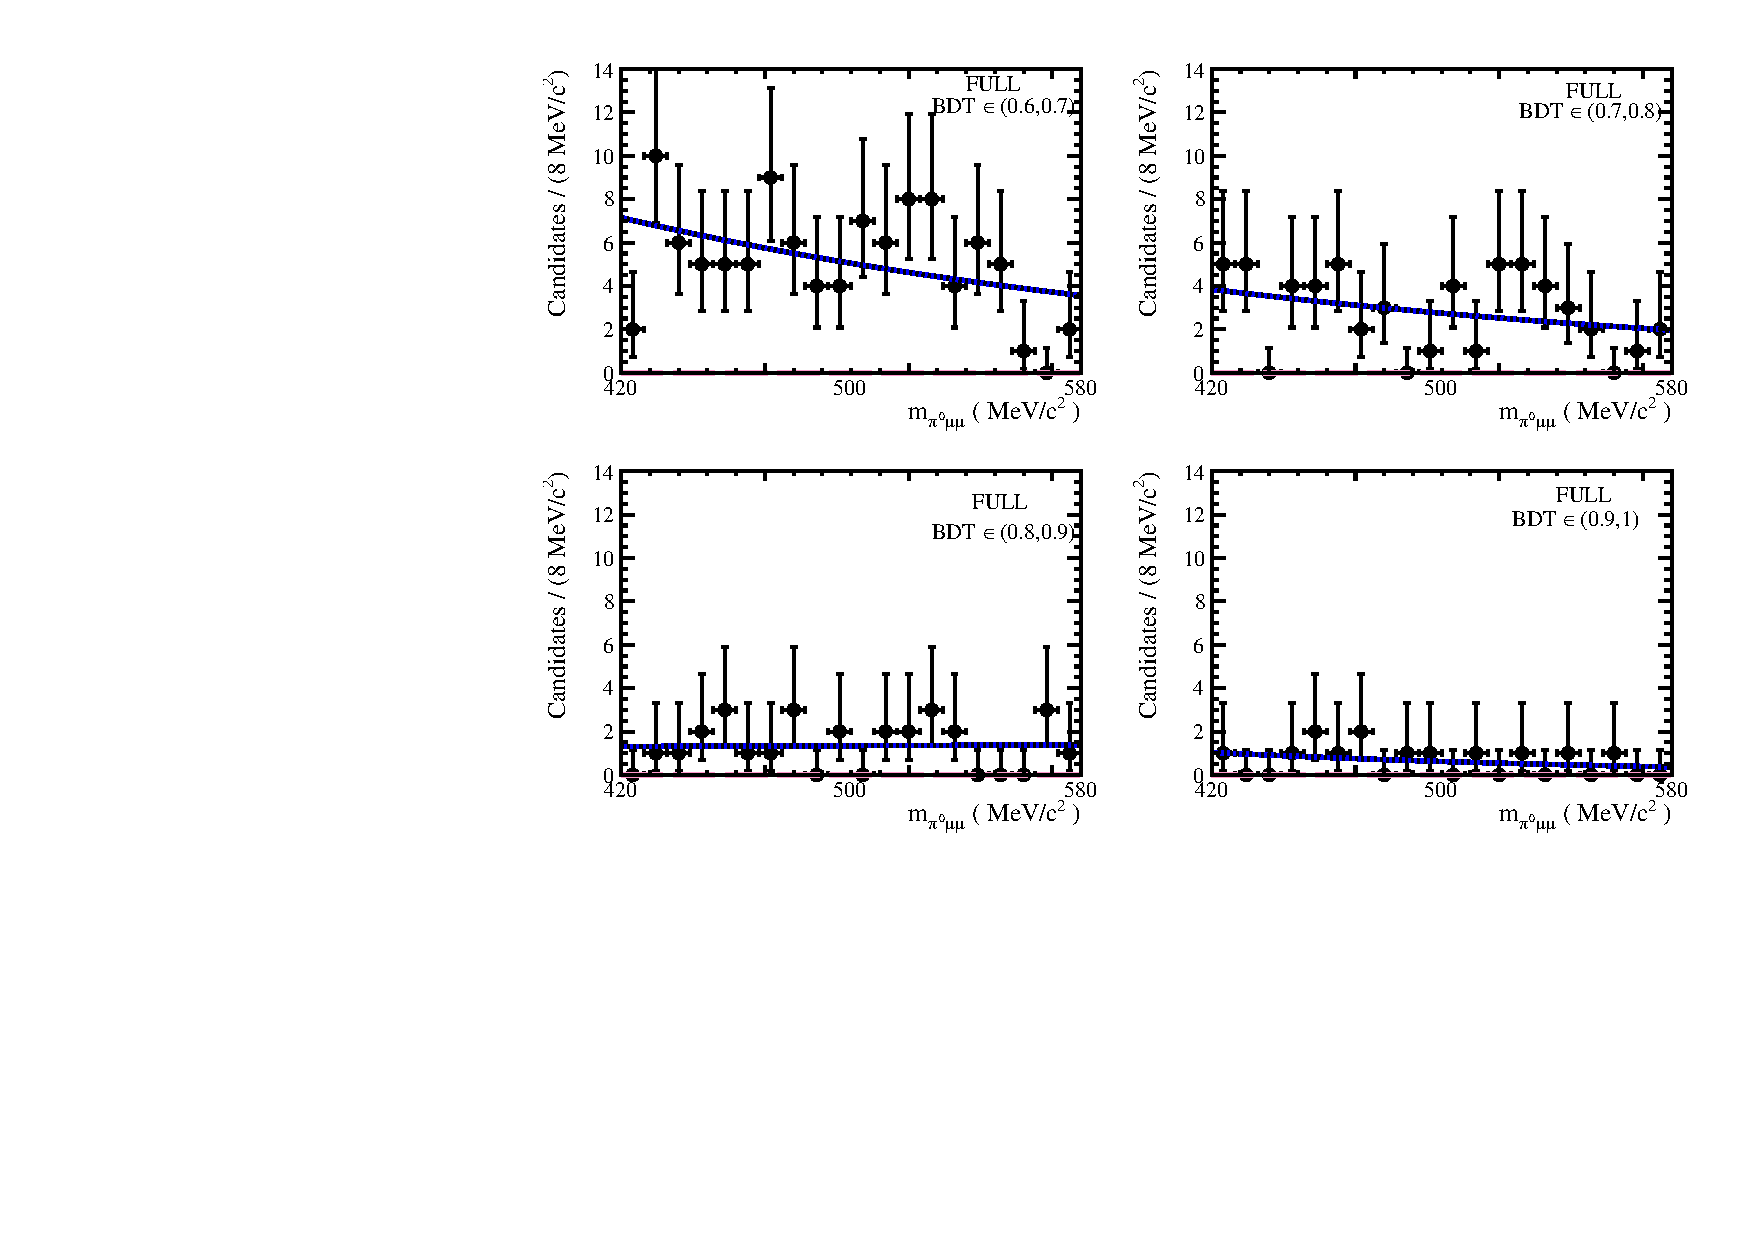
\includegraphics[scale=0.60]{figs/Kspi0MuMu/fit_FULL.pdf}
%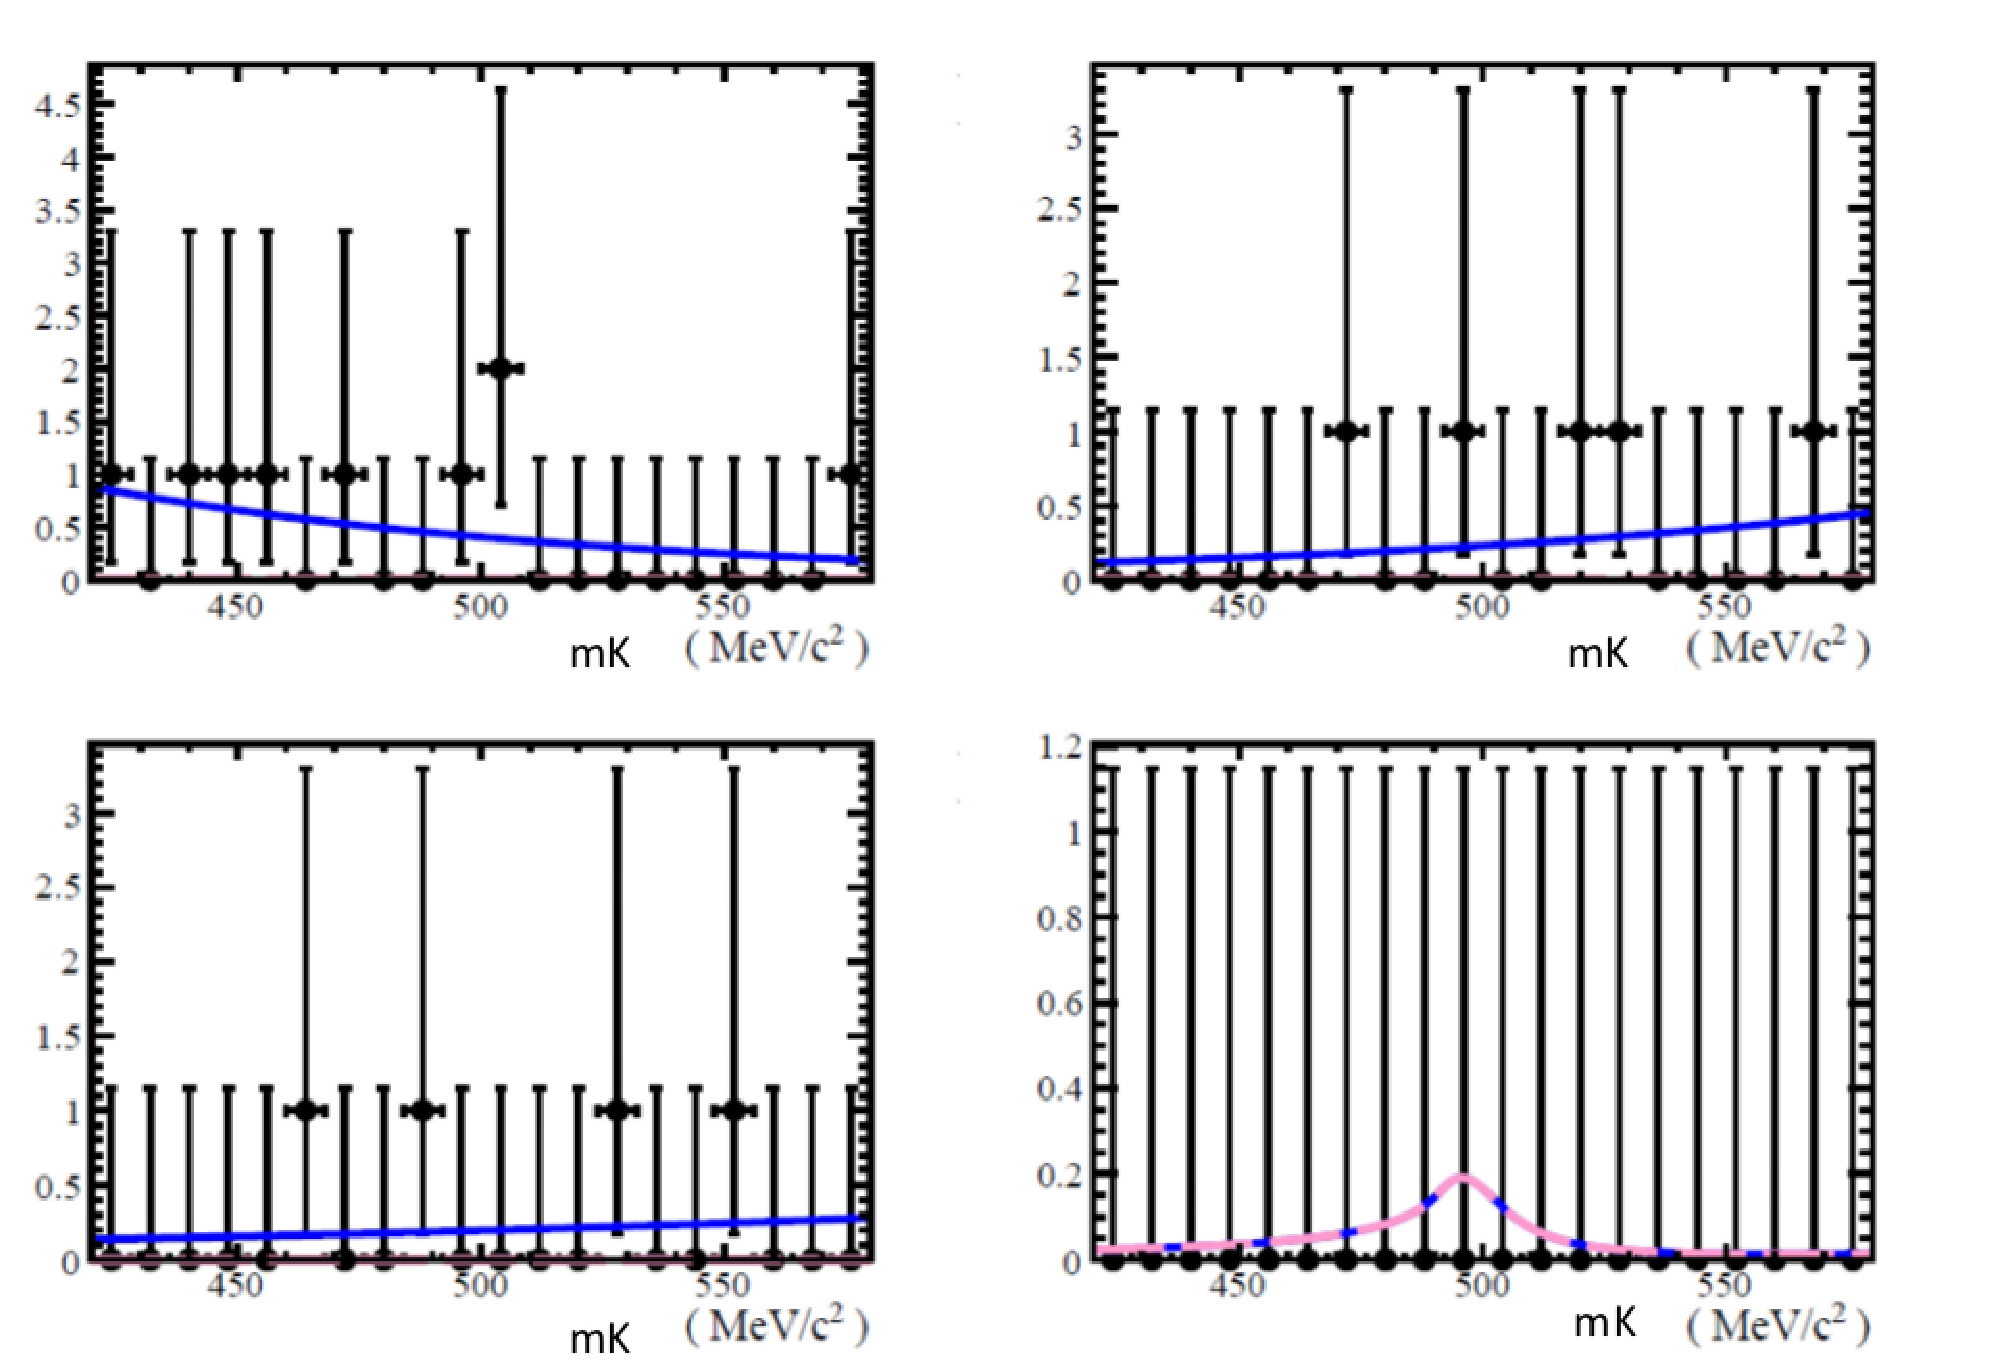
\includegraphics[scale=0.20]{figs/fit_15.pdf}
\includegraphics[scale=0.60]{figs/Kspi0MuMu/fit_PARTIAL.pdf}

\caption{Fit to data for FULL (top) and PARTIAL (bottom) categories. The magenta dashed line shows the signal contribution, the dotted black line the background, and the solid blue line the prediction from the total fit
model.
\label{fig:fit}}
\end{center}

\end{figure}

%\begin{figure} [htb!]
%\begin{center}
%%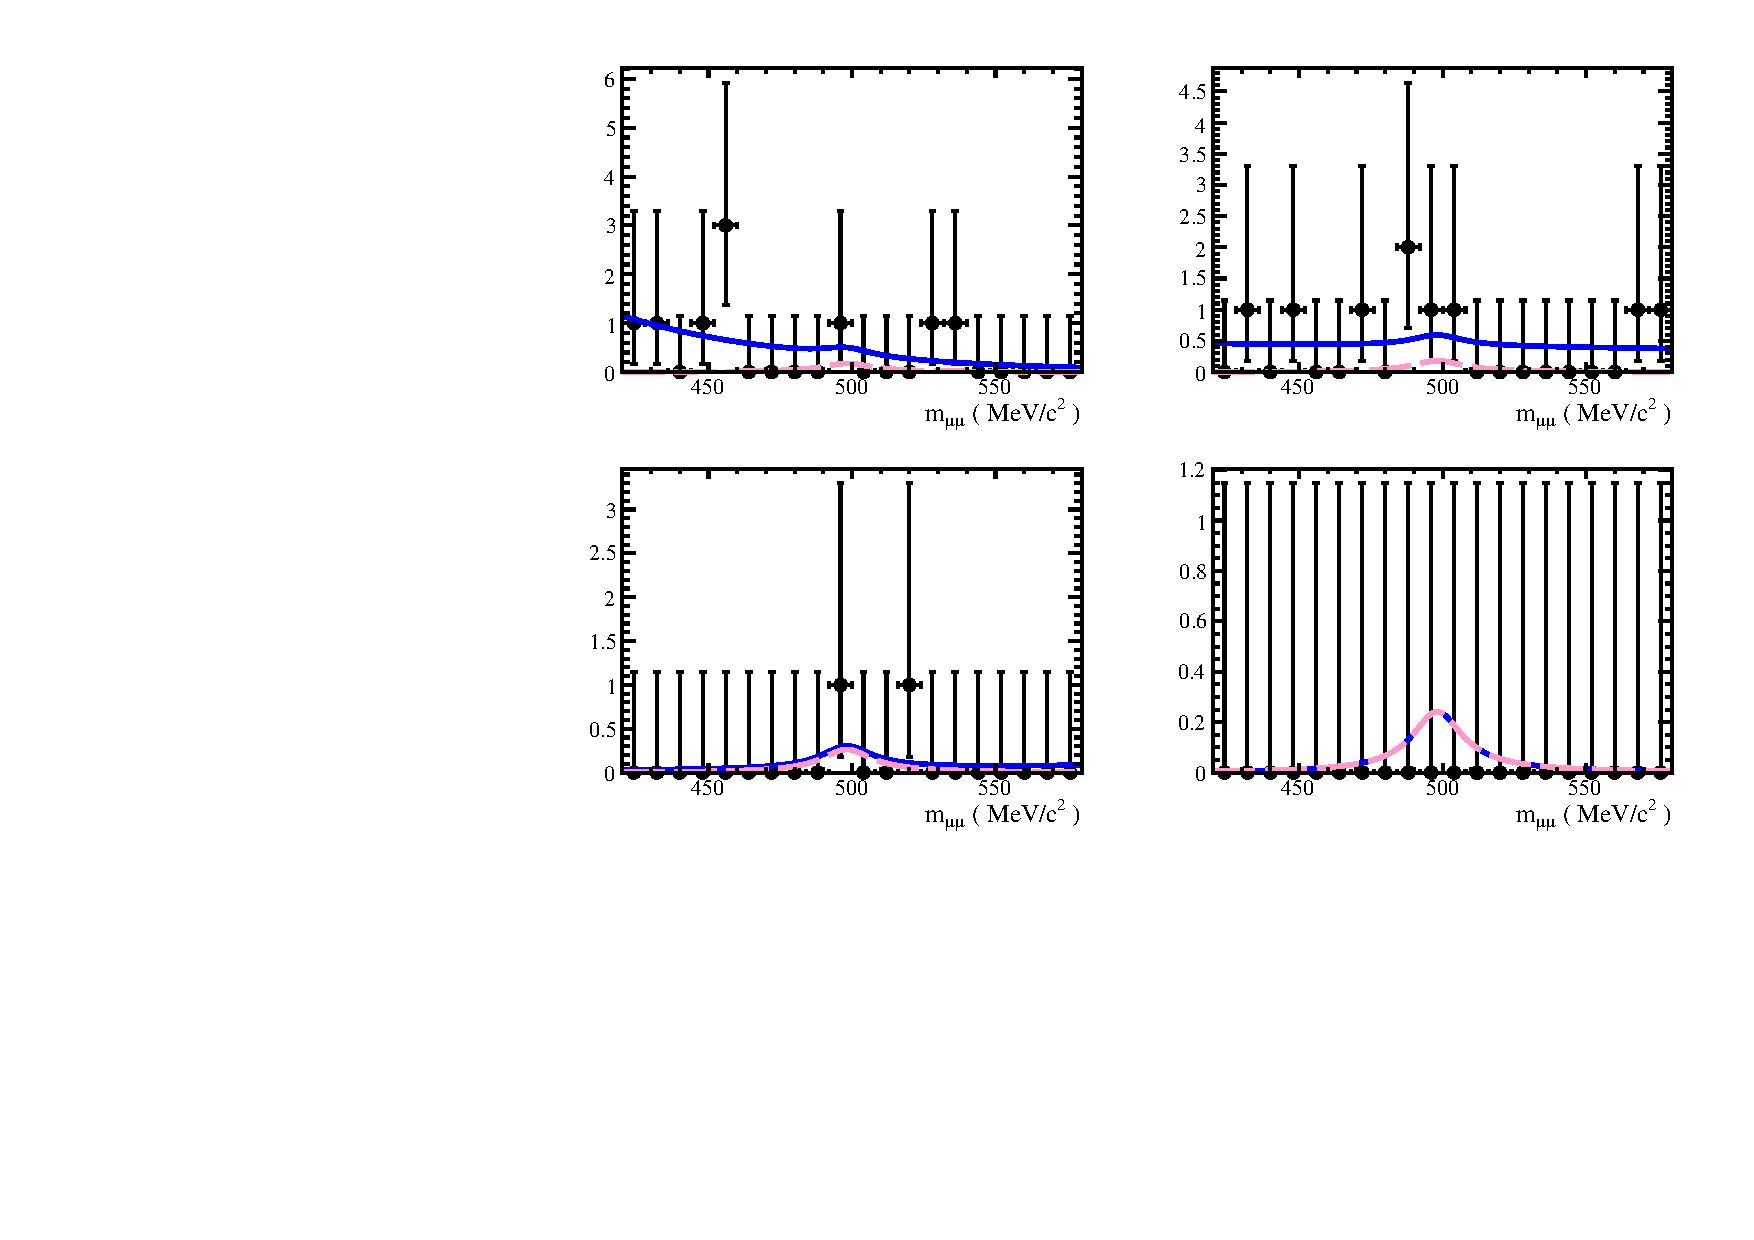
\includegraphics[scale=0.60]{figs/fit_kpmm.pdf}
%\includegraphics[scale=0.60]{figs/fit_PARTIAL.pdf}
%\caption{Fit to data for PARTIAL category. \label{fig:fitPARTIAL}}
%\end{center}
%\end{figure}


%\begin{itemize}
%\item For FULL, we find that the peak shape can be effectively described considering only the 
%resolution parameters
%\end{itemize}
